\documentclass[tikz, border=2pt]{standalone}
\usepackage{tikz}
\usepackage{pgfplots}
\usetikzlibrary{decorations.pathreplacing,calc}
\def\size{2.6}
\begin{document}
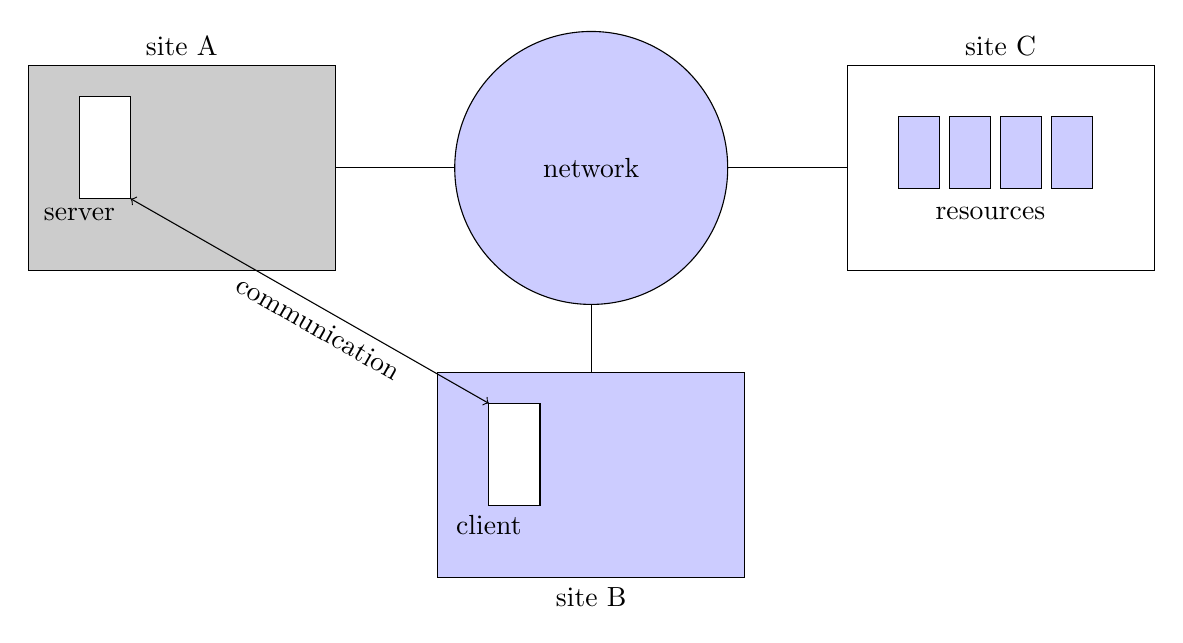
\begin{tikzpicture}
    \coordinate (A) at (-2*\size, 1.5*\size);
    \coordinate (B) at (0,0);
    \coordinate (C) at (2*\size, 1.5*\size);
    \coordinate (N) at (\size*0.75, \size*2);
    \coordinate (server) at ($(A) + (\size*0.25, \size*0.35)$);
    \coordinate (client) at ($(B) + (\size*0.25, \size*0.35)$);
    \draw ($(A) + (\size,0.5*\size)$) -- (N);
    \draw ($(B) + (0.75*\size,\size)$) -- (N);
    \draw ($(C) + (\size,0.5*\size)$) -- (N);
    \draw [fill=blue!20] (N) circle [radius=\size/1.5];
    \draw [fill=black!20] (A) rectangle  ++(\size*1.5,\size);
    \draw [fill=blue!20] (B) rectangle  ++(\size*1.5,\size);
    \draw [fill=white] (C) rectangle  ++(\size*1.5,\size);
    \draw [fill=white] (server) rectangle ++(\size*0.25,\size*0.5); 
    \draw [fill=white] (client) rectangle ++(\size*0.25,\size*0.5);
    \node [below,align=center] at (server) {server};
    \node [below,align=center] at (client) {client};
    \node at (N) {network};
    \draw [<->] ($(client) + (0,\size*0.5)$) -- ($(server) + (\size*0.25,0)$) node [pos=0.45,below,sloped] {communication};
    \node [below] at ($(B) + (\size*0.75,0)$) {site B};
    \foreach \x in {1,...,4} {
        \draw[fill=blue!20] (C) ++(\x*\size/4,\size*0.4) rectangle ++(\size*0.2,\size*0.35);
    }
    \node [above,align=center] at ($(C) + (\size*0.7,\size*0.2)$) {resources};
    \begin{scope}[shift={(\size*1.5/2,\size)}]
        \coordinate (A) at (-2*\size, 1.5*\size);
        \coordinate (B) at (0,0);
        \coordinate (C) at (2*\size, 1.5*\size);
        \node [above] at (A) {site A};
        \node [above] at (C) {site C};
    \end{scope}           
\end{tikzpicture}
\end{document}